La web3 se está desarrollando rápidamente y se espera que cambie la forma en
que interactuamos en línea. Con la tecnología blockchain y los contratos
inteligentes, la web3 permitirá aplicaciones descentralizadas, transacciones
financieras sin intermediarios y la propiedad verdadera de los datos. Algunos
de los protocolos blockchain más populares para la web3 incluyen Ethereum,
Polkadot y Solana.

\hfill \break
Las criptomonedas continúan siendo una fuerza importante en el mercado
financiero global. Bitcoin sigue siendo la criptomoneda más grande y popular,
pero hay muchas otras criptomonedas importantes, como Ethereum, Binance Coin y
Cardano. La capitalización total del mercado de criptomonedas ha aumentado
significativamente en los últimos años, llegando a más de 2 billones de
euros[Figura \ref{fig:capit}] en abril de 2021.
\begin{figure}[htb!]
    \centering
    \caption{Capitalización total del mercado de criptomonedas entre abri del 2017 y mayo de 2023}
    \label{fig:capit}
    \centering
    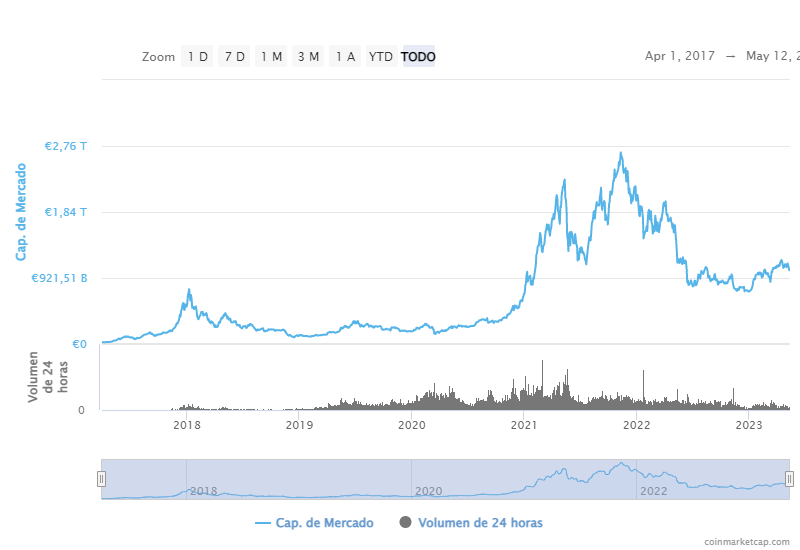
\includegraphics[scale=0.45]{./Ilustraciones/CoinMarketCap chart.png}\\
    \textbf{Fuente:} CoinMarketCap [\url{https://coinmarketcap.com/es/charts/}]
\end{figure}
\hfill \break
Los NFTs se han convertido en un nuevo mercado emocionante en la web3. Las ventas de
NFTs han aumentado significativamente en desde 2020, con algunos NFTs vendiéndose por
decenas de miles de dólares.

\hfill \break
La regulación de las criptomonedas y los NFTs sigue siendo un tema importante.
A medida que estos mercados crecen, los reguladores de todo el mundo están
considerando cómo regularlos para proteger a los inversores y prevenir el
fraude. En algunos países, como China, se han tomado medidas más drásticas para
prohibir las criptomonedas y las transacciones de NFTs.